\documentclass[12pt,a4paper]{article}
\usepackage{amsmath}
\usepackage{tikz}
\usepackage[utf8]{inputenc}
\usepackage{setspace}
\usepackage{subcaption}
\usepackage{geometry}
\usepackage{graphicx}
\usetikzlibrary{shapes.geometric, backgrounds}
\usetikzlibrary{arrows.meta, positioning} % For arrows and 
\usepackage{amssymb}


\usepackage{xcolor}
\usepackage{listings}

\definecolor{gray}{rgb}{0.5,0.5,0.5}
\definecolor{purple}{rgb}{0.58,0,0.82}

% Custom Listings for Binary Blocks
\lstset{
    basicstyle=\ttfamily\small,
    breaklines=true,
    commentstyle=\color{gray},
    keywordstyle=\color{purple},
    stringstyle=\color{purple},
}





\usetikzlibrary{shapes.geometric, arrows, positioning}

\tikzstyle{block} = [rectangle, rounded corners, draw, text centered, minimum width=3.5cm, minimum height=1cm]
\tikzstyle{arrow} = [thick, ->, >=stealth]
\tikzstyle{process} = [rectangle, draw, text centered, minimum width=3.5cm, minimum height=1cm]
\tikzstyle{xor} = [circle, draw, text centered, minimum size=0.6cm]

\usetikzlibrary{positioning} % For node positioning
\usetikzlibrary{calc} % For calculations in TikZ
\usetikzlibrary{math} 
\usetikzlibrary{shapes.geometric, arrows}
\usetikzlibrary{decorations.pathreplacing, arrows.meta}

\tikzstyle{input} = [rectangle, minimum width=2cm, minimum height=1cm, text centered, draw=black, fill=orange!30]
\tikzstyle{function} = [rectangle, rounded corners, minimum width=2.5cm, minimum height=1cm, text centered, draw=black, fill=blue!30]
\tikzstyle{operation} = [rectangle, minimum width=2.5cm, minimum height=1cm, text centered, draw=black, fill=green!30]
\tikzstyle{output} = [rectangle, minimum width=2cm, minimum height=1cm, text centered, draw=black, fill=yellow!30]
\tikzstyle{arrow} = [thick,->,>=stealth]
\definecolor{hotpink}{RGB}{255, 105, 180}
\definecolor{neonyellow}{RGB}{255, 255, 0}
\definecolor{brightorange}{RGB}{255, 165, 0}
\definecolor{brightpurple}{RGB}{128, 0, 128}
\definecolor{turquoise}{RGB}{64, 224, 208}

\usepackage[backend=biber,style=numeric]{biblatex}
\addbibresource{references.bib}


% Page layout
\geometry{top=1in,bottom=1in,left=1in,right=1in}

\begin{document}

\begin{titlepage}
    \centering
    \vspace*{2in}
    
    % Title
    \rule{\textwidth}{0.4pt} \\ % Top horizontal line
    \vspace{0.5cm}
    {\LARGE \textbf{Data Encryption Standard \\
    The Chamber of Secrets: Guarding Digital Realms}} \\
    \vspace{0.5cm}
    \rule{\textwidth}{0.4pt} \\ % Bottom horizontal line
    \vspace{2cm}
    
    % Authors and IDs
    {\large \textbf{Niloy Kumar Mondal} \\
    Student ID: 2105044 \\
    \vspace{0.5cm}
    \textbf{Monjur Hossain Khan Shovon} \\
    Student ID: 2105043} \\
    \vspace{2cm}
    
    % Department and Institution
    {\large Department of Computer Science and Engineering \\ 
    Bangladesh University of Engineering and Technology} \\
    \vspace{2cm}
    
    % Date
    {\large \today}
    
\end{titlepage}



% Table of Contents
\tableofcontents
\newpage

\listoftables
\pagebreak

\listoffigures
\pagebreak

\section{Abstract}
Cryptography is a technique for secure data communication.
Encryption is the process of encoding messages in such a way
that only authorized parties can read it. Decryption is the
process of transforming data that has been rendered
unreadable through encryption back to its unencrypted form.
DES algorithm is a 64 bit block cipher with key of 56 bits. In
this report we will discuss the DES technique for secure data
transmission while maintaining the authenticity and integrity
of the message. In this, message is encrypted before the data
transmission process starts. The encryption and decryption of
data is done by using the data encryption standard algorithm.
\section{Introduction}

This report briefly describes the well known algorithm for Data Encryption process with simulation and example starting from the necessity of data encryption with a story.
\footnote{The story is entirely fictional and used solely for illustrative purposes.}

 \subsection{Problem Definition}
 The Data Encryption Standard (DES) is a symmetric-key block cipher that encrypts data in 64-bit blocks using a 56-bit key, aiming to provide data confidentiality by transforming plaintext into ciphertext. The encryption process involves 16 rounds of permutations and substitutions, producing an encrypted output that can only be decrypted with the correct key.
 
\begin{table}[h!]
\centering
\begin{tabular}{|c|c|}
\hline
\textbf{Input} & \textbf{Output} \\
\hline
Plaintext: 0101010101...010101  & Ciphertext: 3A7BD3A...6A4C99C45 \\
Key: 56 bit Key & \\
\hline

\end{tabular}
\caption{Example of DES Encryption Input and Output}
\end{table}

We want to convert human readable format into unreadable format using a blackbox that will offer reverese extraction of readable format later.

\begin{figure}[h!]
    \centering
    \includegraphics[width=0.8\textwidth]{DataEncryption.png}  % Replace with your image file
    \caption{Comparison of Plaintext and Ciphertext}
    \label{fig:plaintext-ciphertext}
\end{figure}

\subsection{Key Constraints}
\begin{itemize}
    \item  Speed of Encryption and Reversibility 
    \item  Computationally hard backtracking
\end{itemize}




\pagebreak
\section{Motivation}
  Imagine a scenario,Alice wants to send bob some texts.
  If Alice sends it in a simple and understandable format
  in figure \ref{fig:concept1} ,
  there will be a high chances of privace breach over the transmission line.\\ \\
  Can we do better? 
   
\begin{figure}[h!]
    \centering
    \begin{subfigure}[b]{0.48\textwidth}  % Slightly reduce width to fit
        \centering
        \includegraphics[width=\textwidth]{SendingPlainText.png}
        \caption{Sending Plaintext}
        \label{fig:concept1}
    \end{subfigure}
    \hfill
    \begin{subfigure}[b]{0.48\textwidth}  % Slightly reduce width to fit
        \centering
        \includegraphics[width=\textwidth]{SendingEncryptesText.png}
        \caption{Sending Ciphertext}
        \label{fig:concept2}
    \end{subfigure}
    \caption{Comparison between data transmission format}
    \label{fig:motivation}
\end{figure}

If we transmit any permutation of the data, it will be difficult for unauthorized parties or third parties to comprehend the format, even if they gain access to it. At the same time, we must ensure that the actual data can still be extracted. To defend against brute force or backtracking attacks, we should rely on NP-hard
\footnote{NP-hard problems are those for which no known polynomial-time algorithm exists to solve them, and they are at least as hard as the hardest problems in NP.}problems.


\section{Previous Work}

The Data Encryption Standard (DES) has been widely studied since its inception. Rivest (1978) discusses the basic structure and security considerations of DES, highlighting its strengths and limitations in modern cryptography \cite{rivest1978}. Despite being one of the most well-known encryption algorithms, DES has faced criticism over its key length and vulnerability to brute force attacks. In his book, Schneier (1996) provides an extensive overview of cryptographic algorithms, including DES, and discusses various methods to enhance its security \cite{schneier1996}.

Further cryptographic analysis has been conducted to evaluate the security of DES under different attack models. Bellare and Rogaway (1997) presented a comprehensive examination of the security of digital signature schemes, including those based on DES, emphasizing the importance of key management and proper implementation \cite{bellare1997}. Moreover, Bell and Greenberg (1995) provided a cryptographic analysis of DES, focusing on its weaknesses and the potential for cryptanalysis techniques to break the algorithm \cite{des1995}.

These works collectively contribute to understanding the vulnerabilities and strengths of DES, laying the groundwork for the development of more secure encryption standards in the cryptographic community.

\section{Approach}
 \subsection{Algorithm}
   \subsubsection{Overview}
    \begin{itemize}
            \item Symmetric key encryption algorithm.
            \item Operates on 64-bit plaintext blocks.
            \item Uses a 56-bit secret key.
            \item Employs 16 rounds of Feistel network structure.
            \item Ensures data confidentiality through substitution and permutation.
            \item faster runtime
        \end{itemize}
   
   \subsubsection{Visualization of the flow}
   \begin{figure}[h!]
    \centering
    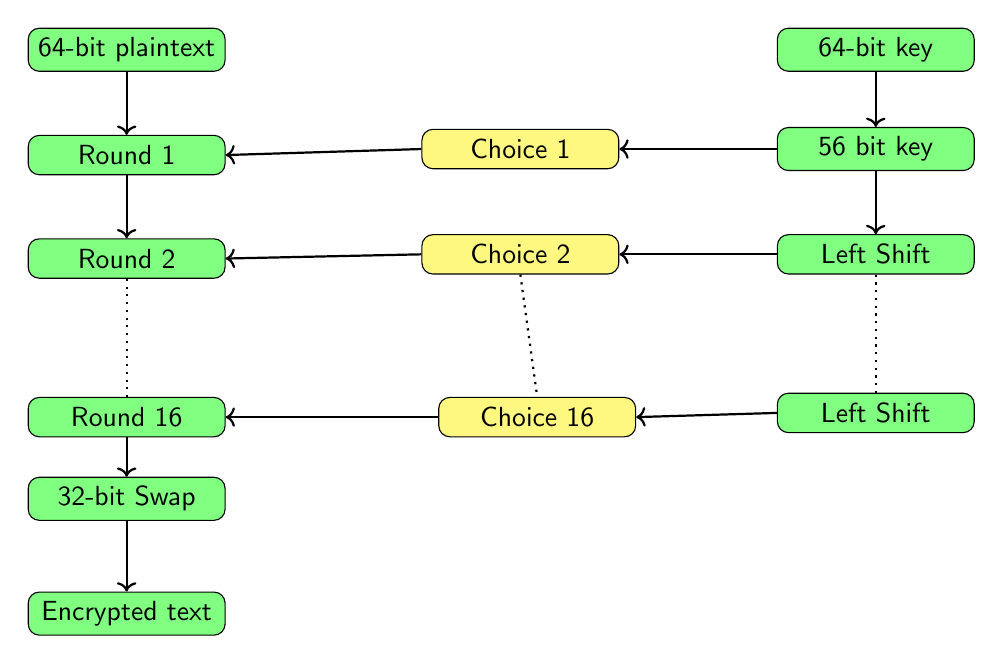
\begin{tikzpicture}[every node/.style={align=center}, 
    arrow/.style={-Triangle, thick}, 
    brace/.style={decorate, decoration={brace, amplitude=5pt}}, 
    custom/.style={
        draw, 
        rounded corners,  
        minimum width=2.5cm, 
        minimum height=0.5cm, 
        font=\sffamily,
        fill=green!50
    }, 
    custom2/.style={
        draw, 
        rounded corners,  
        minimum width=2.5cm, 
        minimum height=0.5cm, 
        font=\sffamily,
        fill=yellow!50
    }]
    
    % Nodes for plaintext and key
    \node[custom] (plaintext) {64-bit plaintext};
    \node[custom, right=7cm of plaintext] (Ikey) {64-bit key};
    
    % Encrypted text node
    \node[custom, below = 6.6cm of plaintext] (ent) {Encrypted text};
    
    % Key transformation nodes
    \node[custom, below=0.7cm of Ikey] (K1) {56 bit key};
    \draw[->, thick] (Ikey.south) -- (K1.north);
    
    \node[custom, below=0.8cm of K1] (K2) {Left Shift};
    \draw[->, thick] (K1.south) -- (K2.north);
    
    \node[custom2, left = 2cm of K1] (c1) {Choice 1};
    \draw[->, thick] (K1.west) -- (c1.east);
    
    % Round 1 node
    \node[custom, below = 0.8cm of plaintext] (r1) {Round 1};
    \draw[->, thick] (plaintext.south) -- (r1.north);
    \draw[->, thick] (c1.west) -- (r1.east);
    
    % Choice 2 node
    \node[custom2, left = 2cm of K2] (c2) {Choice 2};
    \draw[->, thick] (K2.west) -- (c2.east);
    
    % Round 2 node
    \node[custom, below = 0.8cm of r1] (r2) {Round 2};
    \draw[->, thick] (c2.west) -- (r2.east);
    \draw[->, thick] (r1.south) -- (r2.north);
    
    % Round 16 and Choice 16 nodes
    \node[custom, below = 1.5cm of r2] (r16) {Round 16};
    \node[custom2, right = 2.7cm of r16] (c16) {Choice 16};
    \node[custom, below=1.5cm of K2] (K16) {Left Shift};
    
    \draw[dotted, thick] (K2.south) -- (K16.north);
    \draw[dotted, thick] (r2.south) -- (r16.north);
    \draw[->, thick] (c16.west) -- (r16.east);
    \draw[->, thick] (K16.west) -- (c16.east);
    \draw[dotted, thick] (c2.south) -- (c16.north);
    
    % Swap node
    \node[custom, below = 0.5cm of r16] (swap) {32-bit Swap};
    \draw[->, thick] (r16.south) -- (swap.north);
    \draw[->, thick] (swap.south) -- (ent.north);
    
    \end{tikzpicture}
    \caption{DES Algorithm Simulation}
    \label{fig:des_algorithm}
\end{figure}


   \subsubsection{Single round simulation}
   In a single round of the Data Encryption Standard (DES) algorithm, the 64-bit input block is divided into two halves: the left half ($L_i$) and the right half ($R_i$). The right half undergoes a transformation through a function $f$ using a round-specific subkey $K_i$, which is derived from the original key. The left half ($L_i$) is then XORed with the output of the function $f$ and the right half, producing the new right half for the next round ($R_{i+1}$). Simultaneously, the right half becomes the new left half for the next round, while the left half is replaced by the newly computed right half. This process is repeated for 16 rounds, with each round using a new subkey. Finally, after the 16th round, the left and right halves are swapped and combined, and an inverse permutation is applied to generate the ciphertext.

   \begin{figure}
       \centering
        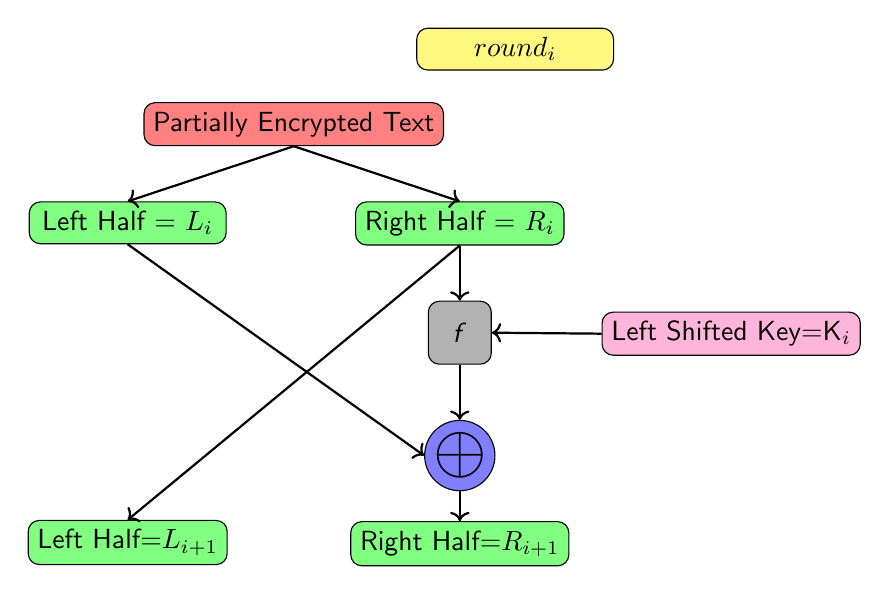
\begin{tikzpicture}[
        every node/.style={
            draw, 
            rounded corners,  
            minimum width=2.5cm, 
            minimum height=0.5cm, 
            font=\sffamily,
            fill=green!50
        },
        round/.style={
            fill=yellow!30 % Light blue background for the 'round' node
        },
        center/.style={
            fill=lightgreen!30 % Light green background for the 'Partially Encrypted Text' node
        }
    ]
        % First row node
        \node[fill=yellow!50](Round) {$round_i$};

        % Partially Encrypted Text
        \node[fill=red!50,below =0.4cm of Round,xshift=-80] (center) {Partially Encrypted Text};

        % Left and Right halves
        \node[below=0.7cm of center, xshift=-60] (left) {Left Half = $L_i$};
        \node[below=0.7cm of center, xshift=60] (right) {Right Half = $R_i$};
        \draw[->, thick] (center.south) -- (left.north);
        \draw[->, thick] (center.south) -- (right.north);

        % Left Half for the next round
        \node[below=3.5cm of left] (left1) {Left Half=$L_{i+1}$};
        \draw[->, thick] (right.south) -- (left1.north);

        % Left Shifted Key
        \node[fill=hotpink!50,below right=2.1 and 2 cm of center] (keys) {Left Shifted Key=K$_i$};

        % f function node
        \node[fill=gray!60,below=0.7cm of right, draw, minimum size=0.8cm, align=center] (function) {\textit{f}};
        \draw[->, thick] (right.south) -- (function.north);
        \draw[->, thick] (keys.west) -- (function.east);

        % XOR operation node
        \node[fill=blue!50,below=0.7cm of function, draw,  shape=circle, minimum size=0.7cm, inner sep=0pt, align=center] (xor) {\Huge $\oplus$};
        \draw[->, thick] (function.south) -- (xor.north);
        \draw[->, thick] (left.south) -- (xor.west);  

        % Right Half for the next round
        \node[fill=green!50,below=3.5cm of right] (right1){Right Half=$R_{i+1}$};
        \draw[->, thick] (xor.south) -- (right1.north);
    \end{tikzpicture}
       
       \caption{Visaulization of single round}
       \label{fig:single-round}
   \end{figure}
   
\pagebreak

 \subsection{Pseudocode}
  
\begin{enumerate}
    \item \textbf{Input:} 64-bit plaintext block \(P\), 64-bit main key \(K\).
    \item Generate 16 round sub-keys \(K_1, K_2, \ldots, K_{16}\) from \(K\).
    \item Apply initial permutation (IP) on \(P\) to get \(L_0\) and \(R_0\).
    \item \textbf{for} \(i \gets 1\) to \(16\) \textbf{do}
    \begin{itemize}
        \item Compute \(L_i \gets R_{i-1}\).
        \item Compute \(R_i \gets L_{i-1} \oplus f(R_{i-1}, K_i)\).
    \end{itemize}
    \item \textbf{end for}
    \item Combine \(R_{16}\) and \(L_{16}\).
    \item Apply inverse initial permutation (IP\(^{-1}\)).
    \item \textbf{Output:} 64-bit ciphertext block \(C\).
\end{enumerate}

 \subsection{Runtime}
 \begin{itemize}
    \item \textbf{Key Generation:}
    The key generation step involves creating 16 sub-keys from the original 64-bit key. This involves shifting the key, performing permutations, and splitting it into two halves. These operations are done for 16 rounds.
    \begin{itemize}
        \item \textbf{Complexity:} Each operation (shifting, permutation) is constant time, i.e., \( O(1) \). Since this process is done 16 times, the total complexity for key generation is \( O(16) = O(1) \).
    \end{itemize}

    \item \textbf{Initial Permutation (IP):}
    The initial permutation is a fixed permutation applied to the 64-bit plaintext.
    \begin{itemize}
        \item \textbf{Complexity:} This is a constant-time operation because the permutation is predefined and applied to a fixed-size block. So, the complexity is \( O(1) \).
    \end{itemize}

    \item \textbf{Rounds (16 rounds):}
    For each of the 16 rounds, the algorithm applies the following operations:
    \begin{itemize}
        \item Splitting the input into two 32-bit blocks.
        \item The \( f \)-function, which involves expansion, substitution, and permutation, all of which take constant time \( O(1) \).
        \item XOR operation with the round key.
        \item A swapping operation (swapping the two halves of the block).
    \end{itemize}
    \begin{itemize}
        \item \textbf{Complexity:} Each round involves a constant number of operations (expansion, substitution, XOR, permutation). Since there are 16 rounds, the total complexity for all rounds is \( O(16) = O(1) \).
    \end{itemize}

    \item \textbf{Final Permutation (IP\(^{-1}\)):}
    The final permutation is similar to the initial permutation and is applied to the result of the 16th round.
    \begin{itemize}
        \item \textbf{Complexity:} This is also a constant-time operation, i.e., \( O(1) \).
    \end{itemize}
\end{itemize}

\textbf{Total Complexity:}
\begin{itemize}
    \item Key Generation: \( O(1) \)
    \item Initial Permutation: \( O(1) \)
    \item Rounds: \( O(1) \) for each round, repeated 16 times: \( O(16) = O(1) \)
    \item Final Permutation: \( O(1) \)
\end{itemize}

Thus, the overall time complexity of the DES algorithm is:
\[
O(1) \text{ (constant time for key generation, permutation, and rounds)}.
\]
\section{Mathmetical Simulation With an Example}
\begin{itemize}
    \item \textbf{64-bit Input Plaintext (Binary):}  
    \begin{lstlisting}
    00101001 00110011 11110000 10101010 
    11001100 11001100 11110000 00000000
    \end{lstlisting}
    \item \textbf{56-bit Key (Binary):}  
    \begin{lstlisting}
    00010011 00110100 01010111 01111001 
    10011011 10111100 11011111 11100001
    \end{lstlisting}
\end{itemize}

\subsubsection*{Step 2: Initial Permutation (IP)}
The 64-bit input undergoes the initial permutation based on the IP table. Each bit is rearranged as specified.

\textbf{Input (Plaintext):}
\begin{lstlisting}
00101001 00110011 11110000 10101010 
11001100 11001100 11110000 00000000
\end{lstlisting}

\textbf{Output After Initial Permutation:}
\begin{lstlisting}
11001100 10101010 11110000 11001100 
11110000 10101010 00110011 00101001
\end{lstlisting}

\subsubsection*{Step 3: Splitting the Block}
The 64-bit permuted block is divided into two 32-bit halves:
\[
L_0 = \texttt{11001100 10101010 11110000 11001100}, \quad 
R_0 = \texttt{11110000 10101010 00110011 00101001}
\]

\subsubsection*{Step 4: Key Scheduling}
The 56-bit key is used to generate 16 round keys \( K_1, K_2, \dots, K_{16} \) through permutation and left shifts.

\textbf{Key Input:}
\begin{lstlisting}
00010011 00110100 01010111 01111001 
10011011 10111100 11011111 11100001
\end{lstlisting}

\textbf{Example Round Key \( K_1 \):}
\begin{lstlisting}
11110000 11001100 10101010 11110000 
\end{lstlisting}

\subsubsection*{Step 5: 16 Rounds of Feistel Function}
Each round applies the Feistel function \( F \), which includes expansion, substitution (using S-boxes), and permutation.

\paragraph{Round 1 Example:}
\begin{itemize}
    \item \textbf{Input:}  
    \( L_0 = \texttt{11001100 10101010 11110000 11001100} \),  
    \( R_0 = \texttt{11110000 10101010 00110011 00101001} \)
    \item \textbf{Key:} \( K_1 = \texttt{11110000 11001100 10101010 11110000} \)
    \item \textbf{Expansion (E):} \( R_0 \) expanded to 48 bits.
    \item \textbf{Feistel Output:} \( F(R_0, K_1) = \texttt{01101010 10111011 11010010 11101010} \)
    \item \textbf{New Values:}
    \[
    L_1 = R_0, \quad 
    R_1 = L_0 \oplus F(R_0, K_1)
    \]
\end{itemize}

\textbf{Output after Round 1:}
\begin{lstlisting}
L_1 = 11110000 10101010 00110011 00101001
R_1 = 10100110 00010001 00100010 00100110
\end{lstlisting}

\subsubsection*{Step 6: Final Permutation (FP)}
After 16 rounds, the left and right halves are concatenated and subjected to the Final Permutation (FP).  

\textbf{Output Ciphertext:}
\begin{lstlisting}
10000101 11101000 00010010 10101101 
00000001 00101011 10101101 01100000
\end{lstlisting}

\subsection*{Summary}
The DES algorithm transforms the 64-bit plaintext into a secure 64-bit ciphertext after 16 rounds of processing.

\textbf{Results:}
\begin{itemize}
    \item \textbf{Input Plaintext (Binary):}  
    \begin{lstlisting}
    00101001 00110011 11110000 10101010 
    11001100 11001100 11110000 00000000
    \end{lstlisting}
    \item \textbf{Input Key (Binary):}  
    \begin{lstlisting}
    00010011 00110100 01010111 01111001 
    10011011 10111100 11011111 11100001
    \end{lstlisting}
    \item \textbf{Output Ciphertext (Binary):}  
    \begin{lstlisting}
    10000101 11101000 00010010 10101101 
    00000001 00101011 10101101 01100000
    \end{lstlisting}
\end{itemize}


\section{Application}
\begin{itemize}
    \item \textbf{Secure Communications}: DES was widely used in securing communications for government organizations, military agencies, and financial institutions.
    \item \textbf{Financial Transactions}: DES was employed in securing electronic payment systems, including ATMs and point-of-sale terminals, as well as protecting financial data during transmission.
    \item \textbf{Data Integrity and Authentication}: DES was used in conjunction with other cryptographic mechanisms like DES-MAC to ensure data integrity and authentication during transmission.
    \item \textbf{Legacy Systems}: Many older systems still use DES for compatibility reasons, often combined with other encryption techniques such as Triple DES (3DES) for enhanced security.
    \item \textbf{Government and Military Applications}: DES was adopted by the U.S. government and military for encrypting sensitive communications and protecting classified information.
\end{itemize}

\section{Challanges and Limitations}
\begin{itemize}
    \item \textbf{Short Key Length:} The 56-bit key length is considered too short for modern security requirements.
    
    \item \textbf{Vulnerability to Brute-Force Attacks:} DES can be cracked in less than 24 hours with modern computational techniques.
    
    \item \textbf{Limited Security Against Cryptanalysis:} DES is susceptible to advanced cryptanalytic techniques, such as differential cryptanalysis.
    
    \item \textbf{Small Block Size:} The 64-bit block size may lead to repeated ciphertext patterns, especially in large datasets.
    
    \item \textbf{Not Suitable for Large-Scale Systems:} The limitations of DES make it unsuitable for use in large-scale or high-security systems.
    
    \item \textbf{Outdated for Modern Applications:} DES has been replaced by more secure algorithms, such as AES, due to its insufficient security for contemporary applications.
\end{itemize}
\section{Conclusions}
 \subsection{Relative comparison and summary}

\begin{table}[h!]
\centering
\begin{tabular}{|c|c|c|}
\hline
\textbf{Feature}               & \textbf{DEA}  & \textbf{DES} \\ \hline
Key Length                     & 56-bit        & 56-bit        \\ \hline
Block Size                     & 64-bit        & 64-bit        \\ \hline
Brute-Force Resistance         & Low           & Low           \\ \hline
Cryptanalysis Resistance       & Weak          & Moderate      \\ \hline
Algorithm Design               & Simple        & Complex       \\ \hline

\end{tabular}
\caption{DEA vs DES Comparison}
\label{tab:des_dea_comparison}
\end{table}
 \subsection{Future of DES}
  DES was a pioneering encryption standard, but it is now considered outdated due to its vulnerabilities. Its limitations led to the development of stronger algorithms, such as AES, which provide better security. As we move forward, the focus is shifting toward post-quantum cryptography, with continuous advancements needed to secure data in an increasingly digital world.

\printbibliography
\end{document}